\chapter{Intelligenza artificiale e apprendimento automatico}
\chaptermark{Apprendimento automatico}
\label{chap:AI_ML}

% \emph{Intelligenza artificiale}, è un'etichetta generica associata a tutti quei sistemi hardware e software in grado di eseguire compiti normalmente svolti da umani, perché richiedono un certo grado di intelligenza umana. 
% Capire cosa è intelligente è necessario per completare la definizione precedente, ma non è un compito facile. 
% Esistono diverse definizioni di intelligenza, ognuna apparentemente più adatta ad un contesto specifico, ma non esiste una definizione universale. 
% L'argomento trattato in questa tesi rientra nel campo dell'intelligenza artificiale, ma più precisamente rientra nel campo del \textit{machine learning}, in italiano apprendimento automatico.

% Risolvere un problema utilizzando un computer, richiede un algoritmo, una sequenza di passi da poter implementare ed eseguire. 
% Per alcuni problemi sono noti uno o più algoritmi in grado di trovare soluzioni: per esempio ordinare una sequenza di numeri è un compito per cui sono noti diversi algoritmi. 
% Per alcuni problemi, invece, conosciamo i dati in input, i dati in output, ma non conosciamo la procedura per trasformare da input in output. 
% Quali sono i passi per considerare un'\textit{e-mail} come posta indesiderata? 
% In caso esistano, sono passi applicabili per ogni casella di posta elettronica? 
% Questi criteri cambiano nel tempo o restano fissi? 
% Per un essere umano identificare un messaggio come indesiderato è relativamente facile; per un \emph{computer} no.

% Il fatto che non siamo in grado di identificare manualmente le caratteristiche che rendono una \textit{e-mail} indesiderata, non vuol dire che queste caratteristiche non esistano. 
% Ci sono, ma sono ``nascoste'' tra i dati. 
% L'\emph{apprendimento automatico} è una branca dell'intelligenza artificiale che studia tutti quei sistemi in grado di apprendere autonomamente analizzando insiemi di dati, per poi eseguire delle predizioni accurate su dati mai visti prima. 
% Oltre alla caratteristica di risolvere compiti che richiedono intelligenza, le tecniche di apprendimento automatico possono prevedere il loro continuo miglioramento, adattando i modelli nel tempo.
% Un modello in grado di identificare posta indesiderata può essere aggiornato nel tempo, aggiungendo nuovi esempi di \emph{e-mail} da scartare.

% Lo studio dei modelli di apprendimento automatico si concentra su due compiti principali: definire procedure di addestramento e definire procedure di inferenza. 
% In genere l'obiettivo principale è quello di costruire dei modelli efficaci, in grado di eseguire predizioni affidabili secondo delle metriche definite in base al problema trattato. 
% In altri scenari, caratterizzati da una scarsità di risorse sia computazionali che temporali, è invece necessario enfatizzare l'efficienza del modello in fase di predizione, idealmente senza sacrificare buone capacità di inferenza.

% Vengono descritte in questo capitolo le caratteristiche e il funzionamento dei più noti algoritmi di apprendimento automatico.

\section{Apprendimento automatico}\label{sec:apprendimento_automatico}
% Ipotizziamo che esista la funzione $f:\mathcal{X}\rightarrow\mathcal{Y}$ ignota. 
% Un algoritmo di apprendimento automatico costruirà un modello $\hat{f}:\mathcal{X}\rightarrow\mathcal{Y}$ che approssima $f$ a partire da un insieme di dati di addestramento, $\mathcal{S}=\{(x_i, y_i)\}$, dove $\mathcal{S} \subset \mathcal{X} \times \mathcal{Y}$. 

% Si parla di \emph{apprendimento supervisionato} quando l'algoritmo di apprendimento richiede la presenza delle etichette $y_i$; si parla di \emph{apprendimento non supervisionato} in caso contrario.
% Si menziona per completezza l'esistenza di una terza categoria, l'\emph{apprendimento per rinforzo}, che include algoritmi che cercano di costruire degli \emph{agenti intelligenti} che identificano la miglior sequenza di operazioni seguendo dei meccanismi di ricompensa e penalizzazione. 
% Gli agenti stessi possono avere un effetto nel ``mondo'' in cui stanno operando, modificando la scelta delle operazioni da compiere.

% Un altra possibile suddivisione dei problemi di addestramento automatico è quella in problemi di classificazione e problemi di regressione.
% Per un problema di regressione le etichette $y_i$ assumono valori continui, mentre per un problema di classificazione le etichette $y_i$ assumono valori discreti. 
% Predire il prezzo di vendita di un immobile a partire dalle sue caratteristiche è un problema di regressione, perché il prezzo di vendita è un valore continuo;
% identificare se un immagine contiene un gatto oppure no è un problema di classificazione, perché la predizione è un valore discreto uguale a ``vero'' oppure ``falso''.

% I problemi di classificazione sono a loro volta ulteriormente divisi in base alla forma delle etichette. Si identificano:
% \begin{itemize}
%     \item Problemi di classificazione binaria: la predizione è una sola etichetta tra due possibili etichette, per esempio $\mathcal{Y} \in \{-1,1\}$.
%     \item Problemi di classificazione \emph{multi-class}: la predizione è una sola etichetta tra molteplici possibili etichette, ovvero $\mathcal{Y} \in \{-1,1\}$
%     \item Problemi di classificazione \emph{multi-label}: la predizione è una o più etichette tra molteplici possibili etichette. 
% \end{itemize}
% I problemi di classificazione per cui la predizione può essere solamente vero/falso sono chiamati problemi di classificazione binaria. I problemi di classificazione per cui esistono più di due classi ma solo una di queste può essere la predizione sono chiamati \emph{multi-class}. I problemi di classificazione per cui esistono più di due etichette e una predizione può 
% **multi-label, multi class, ecc...**
% Clustering è solo classificazione non supervisionata.

% evaluation dei modelli

\section{Comuni approcci risolutivi}
% In questa sezione si descrivono alcuni comuni algoritmi per risolvere i problemi tipici dell'apprendimento automatico categorizzati nel~\Cref{sec:apprendimento_automatico}. 

\subsection{K-Nearest Neighbors}\label{sec:ml:knn}
% K-Nearest Neighbors (KNN) è un algoritmo di machine learning che può essere utilizzato sia per problemi di classificazione che  per problemi di regressione. L'idea principale è quella di assegnare una classe o calcolare un valore di previsione basandosi sulla vicinanza ai punti dell'insieme di addestramento. 
% Secondo questa caratteristica, così come i modelli \emph{support vector machine}, anche KNN è un \emph{instance based learner}, ovvero un modello composto da un sottoinsieme di dati di addestramento, utilizzati per fare predizioni su nuovi dati.

% Per problemi di classificazione binaria e multi-classe, KNN individua i K punti dati più vicini a un punto sconosciuto $\Vec{x}_\text{new}$. 
% La classe più comune tra i K vicini diventa la classe prevista per il punto $\Vec{x}_\text{new}$. 
% Come riportato nell'esempio in~\cref{fig:knn_example}, se $K=3$ e due vicini appartengono alla classe A e uno alla classe B, il punto sconosciuto verrà classificato come parte della classe A, perché la maggioranza dei $K$ punti vicini appartiene alla classe A.

% \begin{figure}[ht]
%     \centering
%     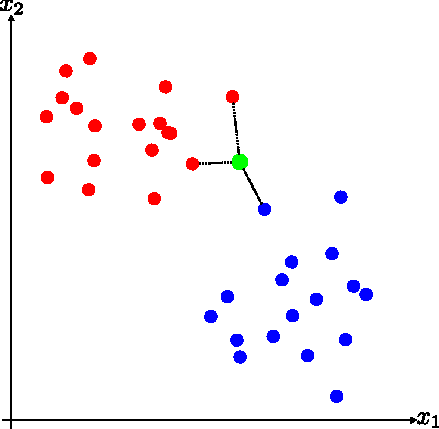
\includegraphics[width=0.5\linewidth]{img/KNN.pdf}
%     \caption{Esempio di applicazione della regola di classificazione KNN con $K=3$. I colori blu e rosso identificano le due possibili classi. Il punto color verde è il punto per cui predire la classe.
%     Il nuovo punto sarà etichettato rosso perché la maggioranza dei punti vicini appartiene a quella classe.}
%     \label{fig:knn_example}
% \end{figure}

% Per problemi di regressione, una volta identificati i K punti più vicini ad $\Vec{x}_\text{new}$, si calcola la predizione come media dei K punti vicini.

% Per addestrare un modello KNN é necessario scegliere un valore di $K$. Un $K$ troppo piccolo porterà a previsioni instabili, mentre un $K$ troppo grande porterà a previsioni troppo generalizzate. Come per altri modelli, potrebbe rendersi necessaria una fase di \emph{model selection} per identificare i migliori iperparametri. In aggiunta a $K$, è necessario definire una misura della distanza tra punti.

% KNN è un algoritmo facile da comprendere e implementare, ma ha delle evidenti limitazioni. 
% \`E sensibile alla scelta di K, ed è particolarmente inadatto per dataset di grandi dimensioni a causa dello spazio richiesto (tutti i dati di addestramento) ma soprattutto per il costo computazionale, dato che è necessario calcolare la distanza rispetto ad ogni elemento per ogni predizione.

% Nonostante queste limitazioni, KNN rimane una scelta valida da utilizzare con dataset di piccole dimensioni.

\subsection{Alberi decisionali}
% Gli alberi decisionali sono modelli che effettuano predizioni basandosi su una struttura dati ad albero creata durante il processo di addestramento. Ogni nodo interno rappresenta una regola, che valutata su un nuovo dato $\Vec{x}_\text{new}$ indicherà in quale sotto-albero procedere con la predizione, fino ad arrivare ad una foglia, che identifica la classe da assegnare. Il processo di addestramento di un albero decisionale identifica quali sono le regole più vantaggiose da utilizzare per raggiungere buone performance di classificazione. L'algoritmo di addestramento più noto è CART. La bontà di ogni decisione viene valutata secondo una metrica, tra le più famose: \emph{Gini impurity}, \emph{information gain} e \emph{root mean squared error (RMSE)}. 
% \begin{figure}[ht]
%     \centering
%     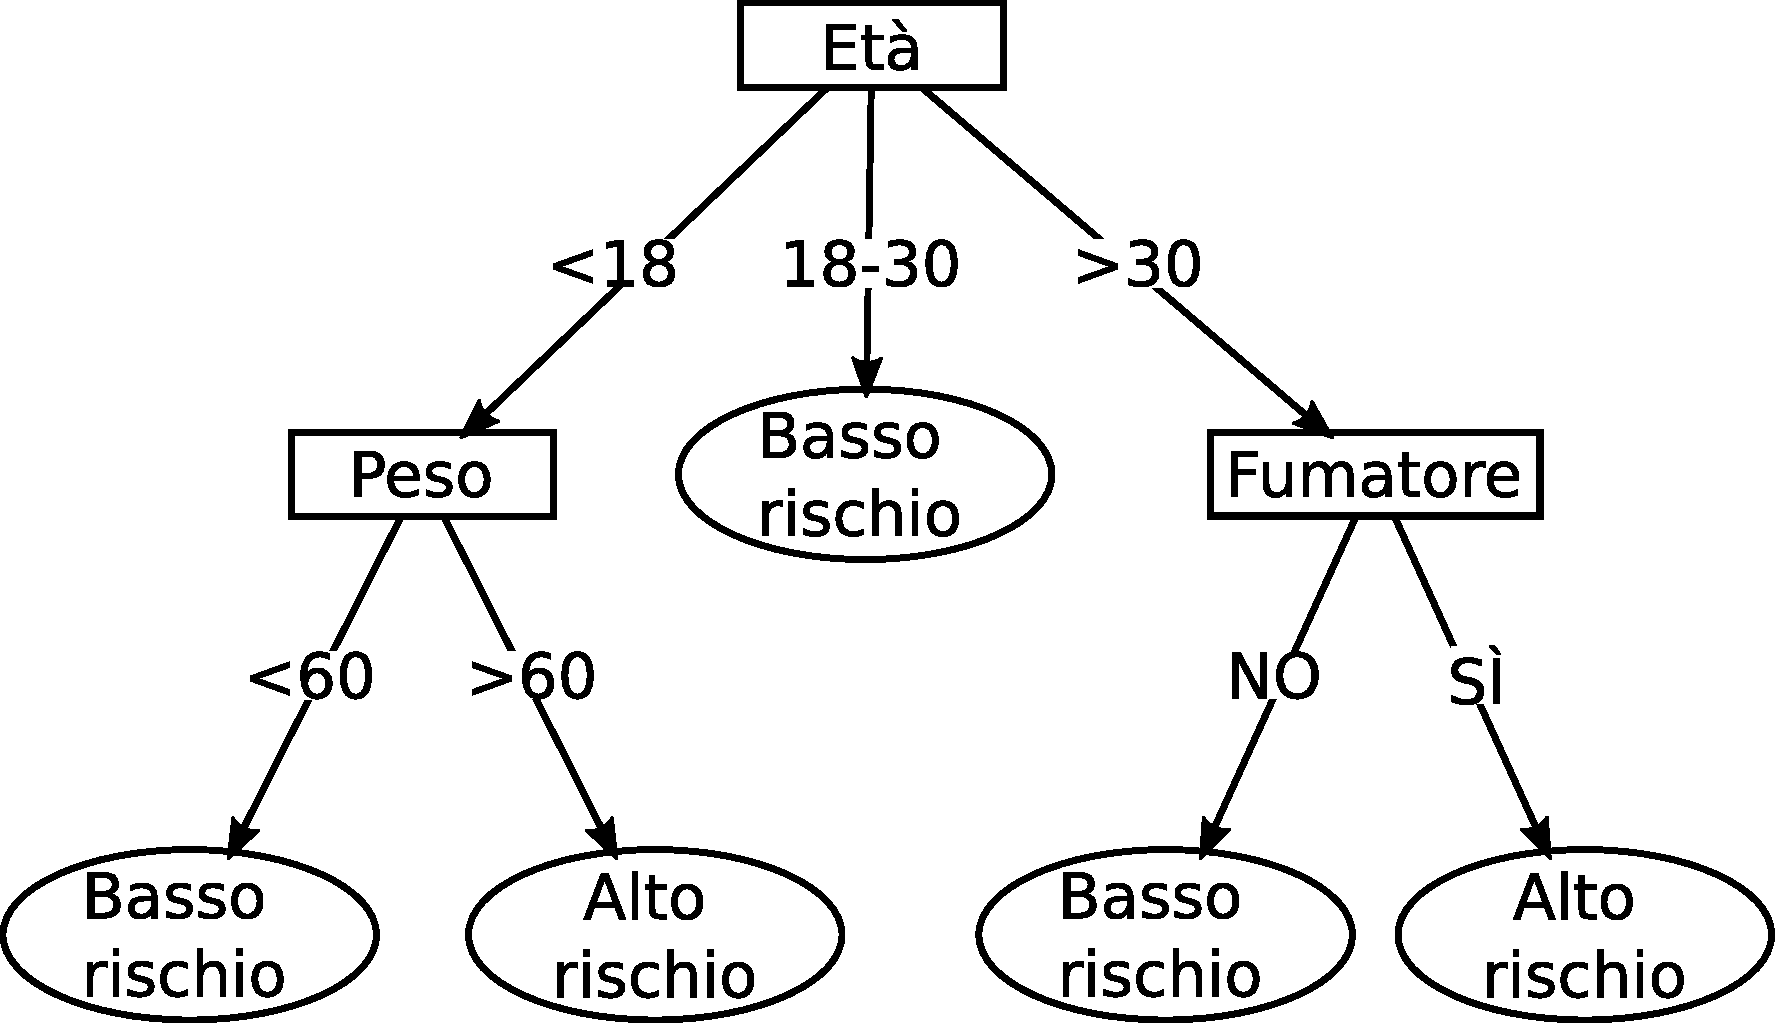
\includegraphics[width=0.5\linewidth]{img/decision_tree.pdf}
%     \caption{Esempio semplificato di un possibile albero di decisione per il rischio di malattia cardiaca. I nodi rettangolari identificano delle regole, in questo caso un semplice controllo sulla \emph{feature} con il nome del nodo. I nodi ovali identificano il valore della predizione.}
%     \label{fig:decision_tree}
% \end{figure}
% Gli alberi decisionali sono modelli semplici e hanno il pregio di essere modelli \emph{white box}, rientrando nei modelli cosiddetti \emph{explainable}.
% Hanno però la tendenza a fare \emph{overfitting}, dato che sarebbe possibile arrivare ad un albero in cui ogni punto di addestramento è una foglia, e soffrono di \emph{variance error}, dato che anche minimi cambiamenti nell'insieme di addestramento potrebbero avere un influenza enorme sul modello prodotto. Per questo motivo, sono molto più utilizzati nella pratica con tecniche di \emph{bagging} e \emph{boosting}. 

\subsubsection{Random Forest}
% \begin{figure}
%     \centering
%     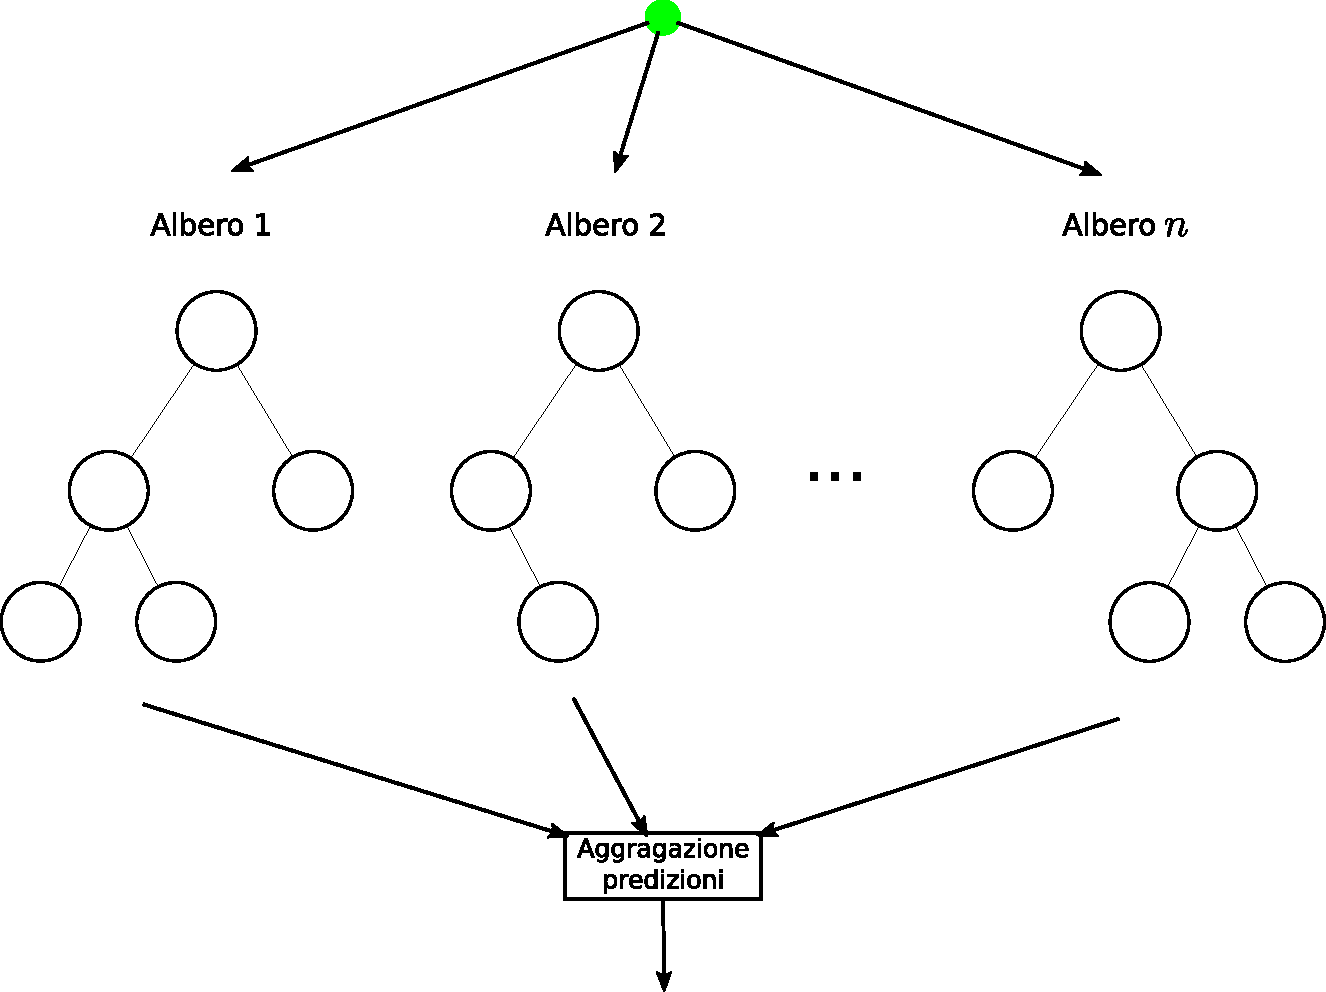
\includegraphics[width=0.5\linewidth]{img/random_forest.pdf}
%     \caption{Esempio di \emph{random forest}. Il modello è composto da un insieme di alberi. Un nuovo esempio da classificare, in questa figura il punto verde, viene classificato da ogni sotto-albero singolarmente, per poi produrre una predizione singola utilizzando una regola di aggregazione delle predizioni interne.}
%     \label{fig:random_forest}
% \end{figure}

%\subsection{Logistic regression}

\subsection{Reti neurali}

% Le reti neurali sono un tipo di modello di apprendimento automatico ispirato alla struttura del cervello umano, composto da neuroni collegati tra di loro ed in grado di scambiare impulsi.
% Nella categoria reti neurali rientra una quantità di modelli molto ampia e estremamente varia.

% Le reti neurali sono nate come estensione del modello \emph{perceptron}~\cite{1958_perceptron}; viene riportato un esempio in~\Cref{fig:perceptron}.
% Un \emph{perceptron} è un modello molto semplice composto da un singolo neurone artificiale.
% Il neurone riceve in ingresso un vettore $\Vec{x}=\{x_1,\dots,x_n\}$ con $x_i \in \mathbb{R}$ ed emette un output 
% \begin{equation*}
%     \hat{y} = \theta\left(\sum_{i=1}^{n}x_iw_i +b\right),
% \end{equation*} 
% dove $w_1,\dots,w_n \in \mathbb{R}$ sono chiamati pesi, $b \in \mathbb{R}$ è il \emph{bias} e $\theta$ è la \emph{funzione di attivazione}, che nel perceptron originale è la \emph{step function} 
% \begin{equation*}
%     \sigma(x) =
%     \begin{cases*}
%       1 & se $x>0$, \\
%       0 & se $x\leq0$.
%     \end{cases*}
% \end{equation*}
% \begin{figure}
%     \centering
%     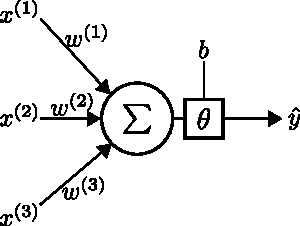
\includegraphics[width=0.5\linewidth]{img/perceptron.pdf}
%     \caption{Esempio di \emph{perceptron}. Le $x_1,x_2,x_3$ identificano gli input, mentre $\hat{y}$ l'output del modello.}
%     \label{fig:perceptron}
% \end{figure}
% Il perceptron è un modello semplice ma è la base per la creazione delle reti neurali.
% Una rete neurale è composta da molteplici \emph{perceptron} collegati tra loro, organizzati in uno o più strati: strato di input, strati nascosti e strati di output.
% Le reti neurali con questa struttura sono anche chiamate \emph{multi-layer perceptron}.
% A seconda del numero di strati nascosti, è possibile dividere le reti neurali come \emph{shallow} o \emph{deep}. Si mostra in~\Cref{fig:NN} un esempio di semplice rete neurale. 
% \begin{figure}
%     \centering
%     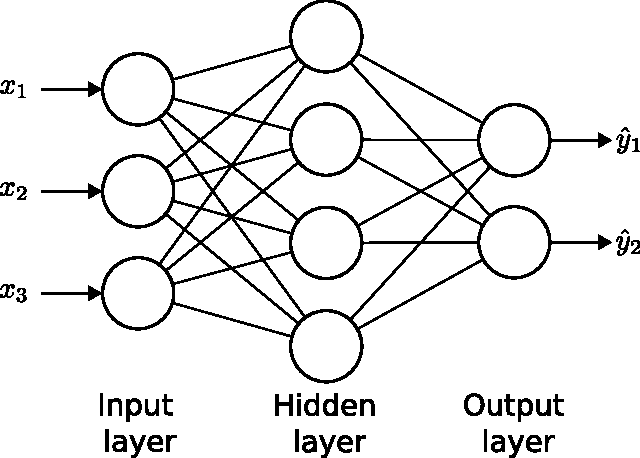
\includegraphics[width=0.5\linewidth]{img/nn.pdf}
%     \caption{Esempio di una semplice rete neurale con 3 neuroni di input e 2 di output.}
%     \label{fig:NN}
% \end{figure}
% Le reti neurali descritte fino ad ora sono chiamate \emph{feed-forward} perché i dati fluiscono dallo strato di input fino a quello di output. 
% Esistono altre tipologie di reti con strutture più complesse, per esempio le reti ricorrenti, le reti convoluzionali, le reti generative e altre numerose varianti e combinazioni. 
% vhk aaaaaafhadvbkflduz kuhxb<kln

% L'addestramento di una rete neurale è effettuato con l'algoritmo di \emph{error backpropagation}.
% In seguito alla fase \emph{forward-pass}, in cui i dati passano nella rete fino a produrre la predizione, viene calcolato l'errore. Percorrendo poi a ritroso la rete nella \emph{backwards-pass}, vengono aggiustati i pesi e i bias dei neuroni.

\section{Bias-variance tradeoff}\label{sec:bias_variance_tradeoff}
% Argomento più in dettaglio in \cite{bias_variance_decomposition}.

% Consideriamo un problema di regressione. Sia $x \in R^p$ una variabile aleatoria di vettori di input e $y \in R$ la variabile aleatoria di valori reali, associati in una distribuzione congiunta $P(X,Y)$ che è ignota. 
% Viene dato $D = \{(x_i,y_i)\}$ dove ogni coppia $(x_i,y_i)$ è estratta a caso da $P$. 
% In genere, si assume che esista una funzione $f$ tale che $Y = f(X) + \epsilon$ dove $\epsilon$ è l'\emph{errore irriducibile}, ovvero un errore che è sempre presente e non dipende dalla bontà del modello predittivo. 
% $\epsilon$ ha media $0$ e varianza $\sigma_\epsilon^2$. L'obiettivo è quello di costruire un predittore (o ipotesi) $\hat{f}$ in grado di approssimare $f$ il meglio possibile. 
% La bontà di un predittore è data dall'errore di predizione. Per problemi di regressione ha senso usare il quadrato della differenza tra predizione e valore effettivo (squared error) come misurazione $Err = E[(Y-\hat{f}(X))^2]$. 
% Per stimare questo errore si usa solitamente un test set, ovvero una porzione di $D$ che non viene usata per il training.
% L'errore di predizione atteso nel punto $x_0$ è quindi $Err(x_0) = E[(Y-\hat{f}(X))^2 | X=x_0]$. Questo errore può essere scomposto in più parti. 
% $$Err(x_0) = \sigma_{\epsilon}^{2}+(E[\hat{f}(x_0)] - f(x_0)])^2 + E[(\hat{f}(x_0) - E[\hat{f}(x_0)])^2]$$
% \begin{itemize}
%     \item \textbf{Errore irriducibile $\sigma_{\epsilon}^{2}$} è la varianza del target attorno alla media effettiva $f(x_0)$.
%     \item \textbf{Bias$^2$} $E[\hat{f}(x_0)]$ è la media tra $\hat{f}_1(x_0), ..., \hat{f}_K(x_0)$, ovvero tutte le possibili predizioni. Bias$^2$ è il quadrato della differenza tra quel valore ed il valore effettivo $f(x_0)$.
%     \item \textbf{Variance} la varianza attesa di $\hat{f}(x_0)$ intorno alla sua media, ovvero la varianza tra $\hat{f}_1(x_0), ..., \hat{f}_K(x_0)$.
% \end{itemize}
% Da questa decomposizione di capisce che l'errore di generalizzazione è influenzato da bias e variance. Un modello con bias alto e variance bassa si dice affetto da underfitting perché non riesce a fare predizioni accurate, anche se queste predizioni sono "vicine". Un modello con variance alta e bias basso si dice affetto da overfitting, perché è molto preciso sui dati di addestramento ma troppo sensibile a testing set diversi e quindi non generalizza bene su dati mai visti.\\
% Si parla di bias variance trade-off perché si osserva spesso che modelli con bias alto hanno variance bassa e viceversa. Un buon predittore è dato dal giusto compromesso tra bias e variance. 

\section{Valutazione dei modelli}
% Nel campo dell'apprendimento automatico è di fondamentale importanza utilizzare delle metriche per misurare l'efficacia dei modelli in fase di addestramento, per poter correggere il procedimento in corso o in ogni caso per quantificare le capacità predittive del modello.
% A prescindere dalla metrica utilizzata, la bontà di un modello è in genere misurata su un \emph{test set}, ovvero un sottoinsieme dei dati disponibili utilizzato solo ed esclusivamente per questo scopo.
% Per una valutazione significativa è necessario un \emph{test set} significativo, composto da un numero sufficiente di elementi e con una distribuzione di etichette il più fedele possibile ad uno scenario reale.
% L'errore principale da evitare nella valutazione di un modello è il così detto \emph{data leakage}. 
% Questo termine identifica tutte quelle situazioni in cui delle caratteristiche che dovrebbero essere ignote al modello in fase di addestramento vengono invece erroneamente utilizzate nell'addestramento.
% Consideriamo per esempio un problema di regressione per cui si vuole predire il valore dello stipendio annuo di alcuni lavoratori a partire da un dataset di caratteristiche rilevanti: se una di queste caratteristiche fosse il valore di stipendio mensile, avremmo una situazione di \emph{data leakage}, perché il dato da predire è sostanzialmente utilizzato dal modello come input.
% Per prevenire queste evenienze ed effettuare buone valutazioni si divide l'insieme di dati disponibile in due parti: un \emph{train set} utilizzato per l'addestramento ed un \emph{test set} utilizzato esclusivamente per la valutazione. **si ma non si fa solo per il data leakage però... vabbè**
% La scelta della composizione del \emph{test set}, come accennato prima, è critica.


% Ipotizzando di avere a disposizione un \emph{test set} di qualità, rimane la scelta di una metrica adatta al modello trattato e quindi adatta ai dati a disposizione: per problemi di classificazione, ad esempio, ha senso utilizzare il numero di predizioni corrette in rapporto al numero di predizioni totali; pre problemi di regressione, invece, non è possibile utilizzare lo stesso criterio perché le predizioni son valori continui e non giusto/sbalgiato. 
% Mentre un classificatore $n$-ario può commettere $n(n-1)$ diversi tipi di errore, denominati \textit{falsi positivi} e \textit{falsi negativi}, nel caso della regressione l'errore può essere un qualunque numero positivo.

\subsection{Metriche per modelli di classificazione}
% Vengono descritte ora le principali metriche per problemi di classificazione.
% Considerando per semplicità un problema di classificazione binaria, si definiscono:
% \begin{itemize}
%     \item \textbf{TP} il numero di predizioni correttamente identificate nella classe positiva.
%     \item \textbf{TN} il numero di predizioni correttamente identificate nella classe negativa.
%     \item \textbf{FP} il numero di predizioni erroneamente identificate nella classe positiva.
%     \item \textbf{FN} il numero di predizioni erroneamente identificate nella classe negativa.
% \end{itemize}
% Queste quantità sono spesso organizzate in una matrice, chiamata \emph{matrice di confusione}.
% Viene riportato in~\Cref{tab:matrice_confusione} un esempio di matrice di confusione per un classificatore binario immaginario che identifica o meno la presenza di una malattia a partire da un referto preso in input.
% \begin{table}[h]
%     \centering
%     \begin{tabular}{l|l|c|c|}
%         \multicolumn{2}{c}{}&\multicolumn{2}{c}{Effettive}\\
%         \cline{3-4}
%         \multicolumn{2}{c|}{} & Positive & Negative\\
%         \cline{2-4}
%         \multirow{2}{*}{Predizioni}& Positive & 1 (TP) & 1 (FP) \\
%         \cline{2-4}
%         & Negative & 8 (FN) & 90 (TN) \\
%         \cline{2-4}
%     \end{tabular}
%     \caption{Esempio di matrice di confusione, da \protect\footnotemark.}
%     \label{tab:matrice_confusione}
% \end{table}

% \footnotetext{\url{https://developers.google.com/machine-learning/crash-course/classification/accuracy?hl=en}}

% \subsubsection{Accuracy} La metrica \emph{accuracy} è una delle metriche principali utilizzate per problemi di classificazione, ed è calcolata come:
% \begin{equation*}
%     \textrm{\emph{Accuracy}} = \frac{\text{Numero di predizioni corrette}}{\text{Numero di predizioni totali}},
% \end{equation*}
% ovvero
% \begin{equation*}
%     \textrm{\emph{Accuracy}} = \frac{\text{TP} + \text{TN}}{\text{TP} + \text{TN} + \text{FP} + \text{FN}}.
% \end{equation*}
% Questa metrica può dare una prima indicazione delle capacità di un classificatore ma può essere poco significativa a seconda del problema considerato, perché non quantifica la distribuzione delle predizioni corrette né la distribuzione di quelle errate.
% Nell'esempio in~\Cref{tab:matrice_confusione} l'accuracy ha valore $0.91$, il che sembrerebbe indicare un buon classificatore.
% Per il problema oggetto dell'esempio però, questo valore è bugiardo, dato che 8 pazienti sarebbero classificati dal modello come in salute quando invece non lo sono: questi 8 errori hanno un costo molto alto per il problema considerato.
% L'accuracy non è sufficiente per valutare questi dettagli.

% \subsubsection{Precision} La metrica \emph{precision}, calcolata come
% \begin{equation*}
%     \textrm{Precision} = \frac{\text{TP}}{\text{TP} + \text{FP}},
% \end{equation*}
% è una misura di quanti degli esempi predetti positivi sono effettivamente positivi. Un modello che predice correttamente tutti gli esempi positivi avrà \emph{precision} 1.
% Nell'esempio in~\Cref{tab:matrice_confusione} il valore di \emph{precision} è $0.5$: quando un paziente è segnalato come ammalato, la predizione è corretta nella metà dei casi.

% \subsubsection{Recall} La metrica \emph{recall}, calcolata come 
% \begin{equation*}
%     \textrm{\emph{Precision}} = \frac{\text{TP}}{\text{TP} + \text{FN}},
% \end{equation*}
% è una misura di quanti veri positivi sono effettivamente identificati come tali.
% Nell'esempio in~\Cref{tab:matrice_confusione} il valore di \emph{recall} è $0.11$: tra tutti gli effettivi pazienti ammalati, il modello ne identifica correttamente l'$11\%$.


% \subsubsection{F1} La metrica F1, calcolata come 
% \begin{equation*}
%     \textrm{\emph{F1}} = \frac{2(\text{\emph{Precision}} \times \text{\emph{Recall}})}{\text{\emph{Precision}} + \text{\emph{Recall}}},
% \end{equation*}
% è una media armonica tra \emph{precision} e \emph{recall}, metriche spesso in contrasto tra di loro. 

\subsection{Metriche per problemi di regressione}
% \subsubsection{\emph{Root mean squared error} (RMSE)}
% \subsubsection{\emph{area under a receiver operating characteristic curve} (AUC)}


\section{Selezione dei modelli}\label{sec:model_selection}
% L'addestramento di un modello di apprendimento automatico richiede il più delle volte la scelta di un valore per alcuni iperparametri. 
% Nel caso dei modelli \emph{k-nearest neighbours} visti nel~\Cref{sec:ml:knn}, per esempio, è necessario fissare un valore per il parametro $k$. 
% La scelta di questi eventuali parametri è di assoluta importanza. 
% Non esiste però in genere una regola fissa ed automatica per fissare a priori un valore soddisfacente: la scelta potrebbe dipendere da tanti fattori, come per esempio dalle caratteristiche dei dati a disposizione, oppure dagli obiettivi desiderati (per esempio potrebbe essere preferibile un modello che genera pochissimi falsi negativi a scapito di più falsi positivi).
% In queste situazioni si utilizzano dei criteri o degli algoritmi per selezionare le migliori combinazioni di iperparametri per il problema da risolvere: questa fase nel processo di creazione di un modelo di addestramento automatico è chiamata \emph{model selection}.
\subsection{Grid Search}
\subsection{Cross Validation}